\def\allfiles{}%允许单文件编译
%专门用于幻灯片制作的beamer文档类
\documentclass[xcolor=table]{beamer}
%在beamer中使用中文
\usepackage[UTF8]{ctex}


%设置主题
\usetheme{CambridgeUS}
\usecolortheme{dolphin}%蓝色

%调用arev宏包修改字体
\usebeamerfont{professionalfonts}
\usepackage{arev}


%列表
\usepackage{enumerate}%有序列表
\usepackage{pifont}%解说列表description


%表格
\usepackage{graphicx}%表格
\usepackage{booktabs, multicol, multirow}%调整表格行高
\usepackage{bigstrut}


%文本框
\usepackage{tcolorbox}
\tcbuselibrary{skins,vignette,raster,listings,listingsutf8,theorems, breakable,magazine,fitting}


%图像处理
\usepackage{graphicx}
\usepackage{float}%允许浮动
\usepackage{caption}%设置标题
\usepackage{graphicx, subfig}


%数学公式
\usepackage{mathtools}%花括号括起的公式


%Tikz绘图
\usepackage{tikz}
\usepackage{pgfplots}



%定理环境
%格式和字体
%\usepackage{theorem}%对定理类环境的进行设置
%\usepackage{ntheorem}%拓展theorem宏包的功能
%\theoremstyle{plain}%定理类环境的格式
%\theorembodyfont{}%定理体字体
%\theoremheaderfont{\heiti}%定理头字体

%自定义定理环境
\newtheorem{defi}{\textbf{定义~}}[section]
\newtheorem{exam}{\textbf{例~}}[section]
\newtheorem{thm}{\textbf{定理~}}[section]
\newtheorem{lem}{\textbf{引理~}}[section]
\newtheorem{cor}{\textbf{推论~}}[section]
\newtheorem{prop}{\textbf{命题~}}[section]
\newtheorem{rem}{\textbf{注~}}[section]


\renewcommand\proofname{\textbf{证明:}}


%自定义宏
\newcommand{\normalfun}[1]
{exp(-x^2/#1)}

\newcommand{\drawfun}[2]
{
		\addplot[
		domain=-3:3,
		samples=200,
		color=#1,
		]
		{#2};
}%前缀
%主文件开始


\begin{document}
%导言区
\title[中国大学生物理学术竞赛]{中国大学生物理学术竞赛介绍}
\subtitle{An Introduction to CUPT}
\author[Ruiyang Zhou]{周锐阳 \\ ruiyangzhou@outlook.com}
\institute[FZU]{物理与信息工程学院 \ \ 福州大学}
\date{2020 年 9 月 22 日}


%封面
\begin{frame}
	\titlepage
\end{frame}


%目录
\begin{frame}{目录}
	\tableofcontents
\end{frame}


%正文
\section{Draw with TeX}
\begin{frame}{Normal Distribution}
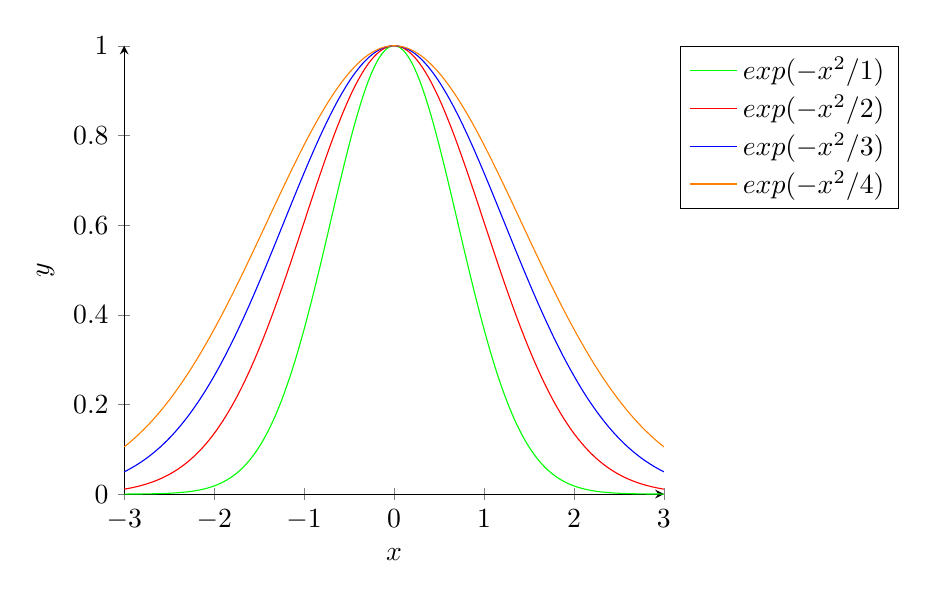
\begin{tikzpicture}
		\begin{axis}[
		legend pos=outer north east,
		axis lines=left,
		xlabel={$x$},
		ylabel={$y$},
		]
\drawfun{green}{\normalfun{1}}
\drawfun{red}{\normalfun{2}}
\drawfun{blue}{\normalfun{3}}
\drawfun{orange}{\normalfun{4}}
\legend{$\normalfun{1}$,$\normalfun{2}$,$\normalfun{3}$,$\normalfun{4}$}
	\end{axis}
\end{tikzpicture}
\end{frame}

\begin{frame}
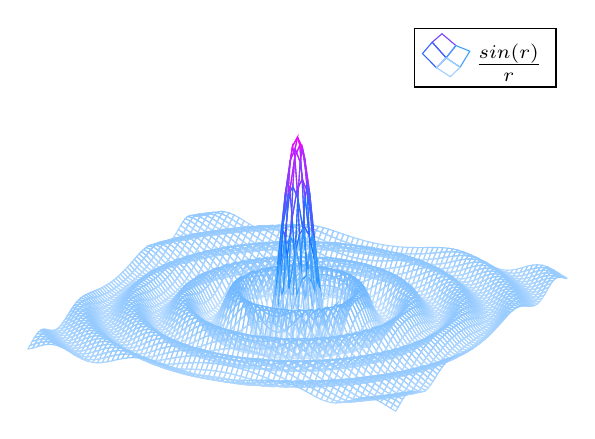
\begin{tikzpicture}
	\begin{axis}[
		hide axis,
		colormap/cool,
		]
		\addplot3[
		mesh,
		samples=75,
		domain=-25:25,
		]
		{sin(deg(sqrt(x^2+y^2)))/sqrt(x^2+y^2)};
		\legend{$\frac{sin(r)}{r}$}
	\end{axis}
\end{tikzpicture}
\end{frame}

\begin{frame}{第二届FZUer的CUPT战绩}

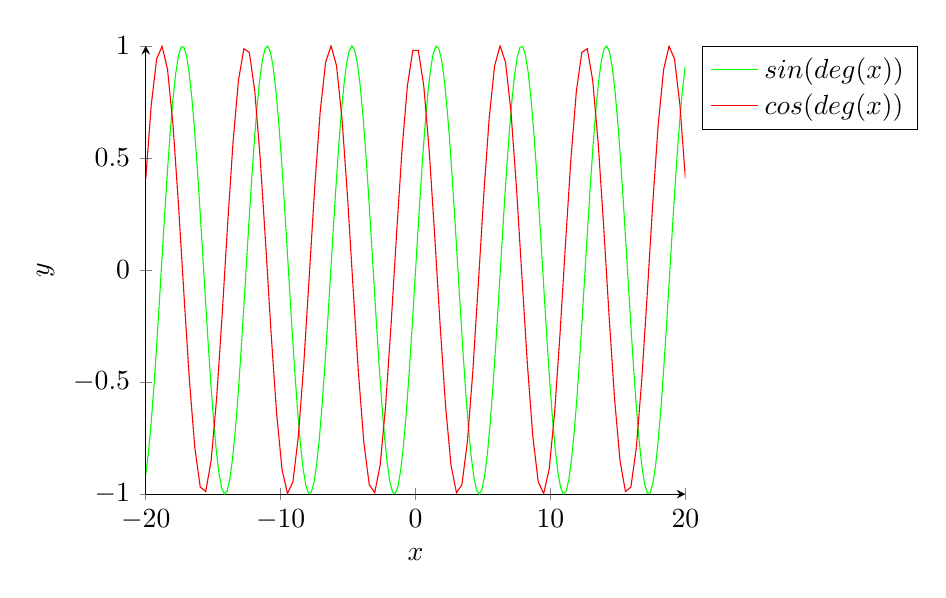
\begin{tikzpicture}
	\newcommand{\f}{sin(deg(x))}
	\newcommand{\g}{cos(deg(x))}
\begin{axis}[
	legend pos=outer north east,
	axis lines=left,
	xlabel={$x$},
	ylabel={$y$},
	]
	
	\addplot[
	domain=-20:20,
	samples=200,
	color=green,
	]
	{\f};
	
		\addplot[
	domain=-20:20,
	samples=100,
	color=red,
	]
	{\g};
	\legend{$\f$,$\g$}
\end{axis}
\end{tikzpicture}





\end{frame}


\begin{frame}

	\begin{center}
		\Huge{感谢聆听！}
	\end{center}
\end{frame}


\end{document}